\documentclass[11pt]{report}

%packages
\usepackage{geometry,
amsmath,
amssymb,
amsthm,
setspace,
mathrsfs,
tikz}

%This is to give color.
\usepackage{xcolor}

%This is to give space on the sides
%and between lines for comments
\geometry{margin=1.in}
%\doublespacing

\theoremstyle{plain}
\newtheorem{thm}{Theorem}
\newtheorem{lem}[thm]{Lemma}
\newtheorem{prop}[thm]{Proposition}
\newtheorem{cor}[thm]{Corollary}

%%%%
%% New Commands
%%%%
\newcommand{\modn}[3]{#1 \equiv #2 \: (\text{mod } #3)}
\newcommand{\Z}{\mathbb{Z}}
\newcommand{\R}{\mathbb{R}}
\newcommand{\N}{\mathbb{N}}
\newcommand{\bs}{$\backslash$}
\newcommand{\ps}{\mathscr{P}}

%%%%%%%
% Document Begins
%%%%%%%%
\begin{document}
\hfill Math 265

%%% Your Name goes HERE
\hfill \textbf{YOUR NAME HERE}

\hfill \today

\begin{center}
\Large{\textbf{Homework \# 11}} \\

\end{center}

\noindent\fbox{Problem List} \\ \S 11.1 \# 1, 2, 6, 10, 15\\
\S 11.2 \# 1, 2, 8, 13\\
\S 11.3 \# 3, 8, 9\\
\S 11.4 \# 3, 5, 6\\
\S 11.5 \# 6, 7\\
\S 12.1 \# 2, 3, 7, 8, 11

\begin{enumerate}
%problem
\item[\textbf{11.1.1}] Let $A = \{0,1,2,3,4,5\}.$ Write out the relation R that expresses $>$ on $A$.\\
\textbf{Answer:} \\
\vspace{0.5in}
%problem
\item[\textbf{11.1.2}] Let $A =\{1,2,3,4,5,6\}.$  Write out the relation R that expresses $\mid$ (divides) on $A.$\\
\textbf{Answer:} \\
\vspace{0.5in}
%problem
\item[\textbf{11.1.6}] Congruence modulo 5 is a relation on the set $A =\Z.$ In this relation $x \:R\: y$ means $$x \equiv y \pmod 5.$$ Write out the set R in set-builder notation.\\
\textbf{Answer:} \\
\vspace{0.5in}
%problem
\item[\textbf{11.1.10}] Consider the subset $R = (\R \times \R)-\{(x, x) : x \in \R\} \subseteq \R \times \R.$ What familiar relation on R is this? Explain.\\
\textbf{Answer:} \\
\vspace{0.5in}
%problem
\item[\textbf{11.1.15}] A subset of $R$ of $\Z^2$ is indicated by gray shading. It is a familiar relation. State it.\\


%%%%%%%%%%%
%% This is the Tikz code
%% that produces the picture
%% once you have your answer
%% you can delete it, if you like
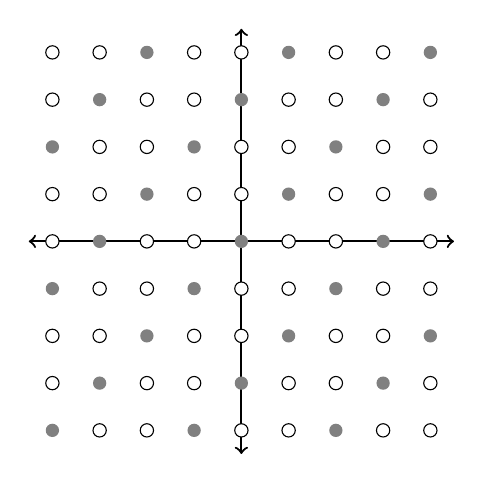
\begin{tikzpicture}[scale=.6]
\draw[thick, <->](-4.5,0)--(4.5,0);
\draw[thick, <->](0,-4.5)--(0,4.5);
\foreach \x in {-4,...,4} {
  \foreach \y in {-4,...,4} {
    \pgfmathtruncatemacro{\diff}{mod(\x - \y, 3)}
    \ifnum\diff=0
      \fill[gray] (\x,\y) circle (4pt);
    \else
      \fill[white] (\x,\y) circle (4pt);
      \draw (\x,\y) circle (4pt);
    \fi
  }
}
\end{tikzpicture}\\
%%%%%%
%% END OF TIKZ code
%%%%%

\textbf{Answer:} \\
\vspace{0.5in}
%problem
\item[\textbf{11.2.1}] Consider the relation $R =\{(a,a),(b,b),(c, c),(d,d),(a,b),(b,a)\}$ on set $A =\{a,b, c,d\}.$ Is R reflexive? Symmetric? Transitive? If a property does not hold, say why.
%problem
\item[\textbf{11.2.2}] Consider the relation $R =\{(a,b),(a, c),(c, c),(b,b),(c,b),(b, c)\}$ on the set $A = \{a,b, c\}.$ Is R reflexive? Symmetric? Transitive? If a property does not hold, say why.
%problem
\item[\textbf{11.2.8}] Define a relation on $\Z$ as $x\:R\: y$ if $|x- y| < 1.$ Is R reflexive? Symmetric? Transitive?
If a property does not hold, say why. What familiar relation is this?
%problem
\item[\textbf{11.2.13}] Consider the relation $R =\{(x, y) \in \R \times \R : x- y \in \Z\}$ on R. Prove that this relation is
reflexive, symmetric and transitive.
%problem
\item[\textbf{11.3.3}] Let $A =\{a,b, c,d, e\}.$ Suppose R is an equivalence relation on A. Suppose R has three equivalence classes. Also $aRd$ and $bRc.$ Write out R as a set and explicitly describe all three equivalence classes.
%problem
\item[\textbf{11.3.8}] Define a relation R on $\Z$ as $xR y$ if and only if $x^2+y^2$ is even. Prove R is an
equivalence relation. Describe its equivalence classes
%problem
\item[\textbf{11.3.9}] Define a relation R on Z as $xR y$ if and only if $4\mid (x+3y).$ Prove R is an equivalence
relation. Describe its equivalence classes
%problem
\item[\textbf{11.4.3}] Describe the partition of $\Z$ resulting from the equivalence relation $\equiv \pmod 4.$
%problem
\item[\textbf{11.4.5}] Consider the partition $P =\big\{ \{...,-4,-2,0,2,4,...\}, \{...,-5,-3,-1,1,3,5,...\} \big\}$ of $\Z.$
Let R be the equivalence relation whose equivalence classes are the two elements
of P. What familiar equivalence relation is R?
%problem
\item[\textbf{11.4.6}] Consider the partition $P =\big\{\{0\}, \{-1,1\}, \{-2,2\},\{-4,4\},\dots \big\}$ of $\Z.$ Describe
the equivalence relation whose equivalence classes are the elements of P.
%problem
\item[\textbf{11.5.6}] Suppose $[a],[b] \in \Z_6$ and $[a]\cdot [b] = [0].$ Is it necessarily true that either $[a] = [0]$ or[$b] = [0]$? What if $[a],[b] \in \Z_7$?
%problem
\item[\textbf{11.5.7}] Do the following calculations in $\Z_9,$ in each case expressing your answer as $[a]$ with $0 \leq a \leq 8.$
	\begin{enumerate}
	\item $[8]+[8]$ 
	\item $[24]+[11]$ 
	\item $[21]\cdot[15]$ 
	\item $[8]\cdot[8]$
	\end{enumerate}
%problem
\item[\textbf{12.1.2}]  Suppose $A =\{a,b,c,d\},$  $B =\{2,3,4,5,6\}$ and $f =\{(a,2),(b,3),(c,4),(d,5)\}.$ State the domain and range of $f.$ Find $f (b)$ and $f (d).$
%problem
\item[\textbf{12.1.3}] There are four different functions $f : \{a,b\} \to \{0,1\}.$ List them
%problem
\item[\textbf{12.1.7}] Consider the set $f =\{(x, y) \in \Z \times \Z : 3x + y = 4\}.$ Is this a function from $\Z$ to  $\Z$?
Explain.
%problem
\item[\textbf{12.1.8}] Consider the set $f =\{(x, y) \in \Z \times \Z : x + 3y = 4\}.$ Is this a function from $\Z$ to $\Z$?
Explain.
%problem
\item[\textbf{12.1.11}] Is the set $\theta =\{(X,|X|) : X \subseteq \Z_5\}$ a function? If so, what is its domain and range?


\end{enumerate}
\end{document}